% mainfile: ../ltexpprt.tex

One of the problems with PAHO count dataset is that PAHO count value of a specific week may change over time. In other words, PAHO count values are unstable for a period of time after they are published for the first time. We can categorize PAHO count values into three different types. The first type, is unknown PAHO counts that we show them by $\ddot{P}_i$ and we want to predict them. The second type is known and stable PAHO counts. We show stable PAHO counts by $\dot{P}_i$. The third type is named as unstable known PAHO counts and are shown by $\tilde{P}_i$. In this section we study the issue of instability in PAHO count values and propose a model to adjust these unstable values to more accurate ones.

In order to study the stability behavior of PAHO data, we start with plotting relative error of PAHO count values with respect to the stable values. Relative error is defined as follows:

\begin{equation}
E_{relative} = \frac{\tilde{P}_i - \dot{P}_i}{\dot{P}_i}
\end{equation}

Average relative error for Argentina and Colombia are illustrated in Figure ~\ref{fig:relerrors}. As it can be seen, different countries have different stability behaviors. On average, for some countries, PAHO count values are stabilized very slowly while for others, they are stabilizing faster. Stability behavior of PAHO count values also depends on time of the year. Figure ~\ref{fig:seasonal_relerrors} shows how average relative error of PAHO count values change over time for Argentina in different influenza seasons of the year. Here we assumed that any time of the year with total PAHO count value less than 100 cases is low season. It is also assumed that when PAHO count is greater than 300 we are in high season and mid season is when PAHO count is between 100 and 300. It worth mentioning that thresholds of low, mid, and high season is different for each country.

% talking about priliminary results
\begin{figure*}[h]
  \centering
   \begin{tabular}{cc}
     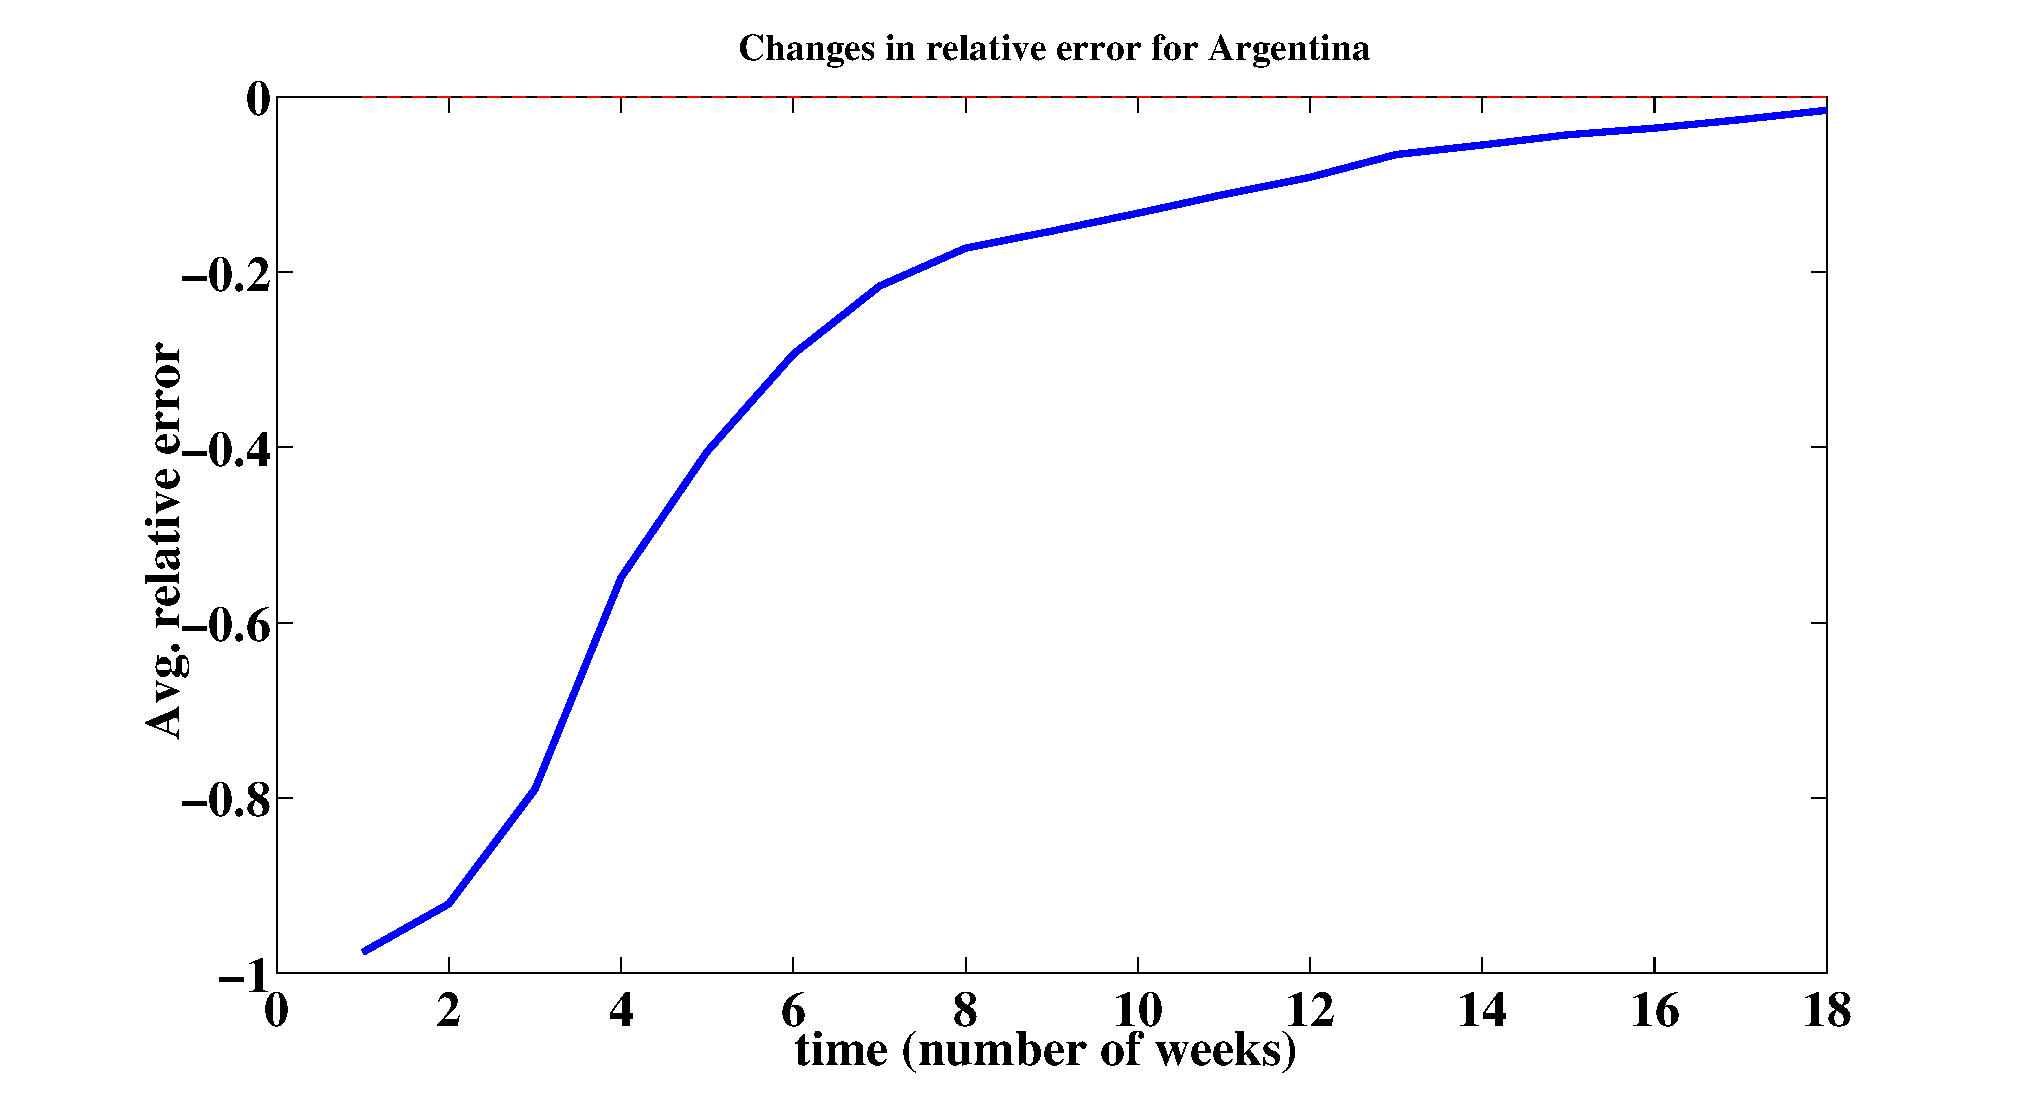
\includegraphics[width=.45\textwidth]{fig/forpaper_AVGrelativeALLs_Argentina.eps} &
     \includegraphics[width=.45\textwidth]{fig/forpaper_AVGrelativeALLs_Colombia.eps} \\
 %    \includegraphics[width=.23\textwidth]{forpaper_AVGrelativeALLs_Ecuador.eps} &
 %    \includegraphics[width=.23\textwidth]{forpaper_AVGrelativeALLs_Mexico.eps} \\
      (a) & (b) \\ %& (c) & (d) \\
  \end{tabular}
  \caption{Average relative error of PAHO count values with respect to stable values.
  (a) Argentina,
  (b) and Colombia.
%  (c) Ecuador, and
%  (d) Mexico.
  }
  \label{fig:relerrors}

\end{figure*}

\begin{figure}[h]
  \centering
    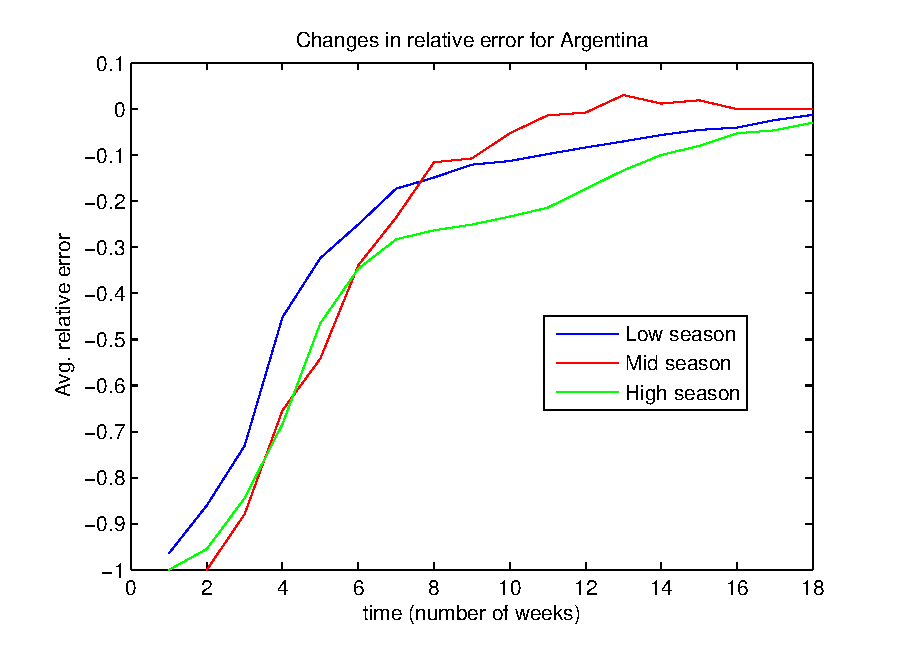
\includegraphics[width=0.8\textwidth]{fig/forpaper_seasonalAVGrelativeALLs_Argentina.eps}
  \caption{Average relative error of PAHO count values for Argentina with respect to their stable values for low, mid, and high seasons.}
  \label{fig:seasonal_relerrors}
\end{figure}  

% waiting for publishing stable PAHO values does not work because it is too late

Based on available dataset and using data analytic methods we can adjust known unstable PAHO counts to have a better estimate of them. Preliminary results show that for different seasons and different countries, we have different stability patterns. Therefore, any PAHO count adjustment method should be customized for seasons and countries separately. 

Let us assume that $\dot{\mathcal{P}}$ is the set of stable PAHO counts for a specific country. Also, assume that sequence of updates for each stable PAHO count value is available. In other words, for $\dot{P}_i$ we have the following set:
 
\begin{equation}
\dot{\mathcal{P}}_i = \left \{P_i^{(1)},P_i^{(2)},...,P_i^{(m)},...  \right \}
\end{equation}

where, $P_i^{(m)}$ is the value of $P_i$ after $m$ time slots (i.e. $m$ weeks). For each stable PAHO count value, $\dot{P}_i$, there is a threshold, $\dot{T}_i$ that for $m \ge \dot{T}_i$, $P_i^{(m)}$ is stable. Hence, we have:

\begin{equation}
\dot{\mathcal{P}}_i = \left \{P_i^{(1)},P_i^{(2)},...,P_i^{(\dot{T}_i-1)},\dot{P}_i,\dot{P}_i,...  \right \}
\end{equation}

In other words, $P_i$ will be stable after $\dot{T}_i$ time slots (weeks). 

After recognizing high, low, and mid-season months for the country, we can categorize each $\dot{P}_i$ to belong to one of these categories. Then, for category S, an adjustment dataset is constructed named as $\mathcal{P}_A{^S}$ which is defined as follows:

\begin{equation}
\mathcal{P}_A{^S} = \left \{ (1,P_i^{(1)},\dot{P}_i),(2,P_i^{(2)},\dot{P}_i),...,(m,P_i^{(m)},\dot{P}_i), ...  \right \}
\end{equation}

Each member of $\mathcal{P}_A{^S}$ is a tuple with three items: first item shows the time slot that the sample belongs to, second item is the actual unstable value of $P_i$, and third item is the related stable value.

In the next step, a linear regression algorithm is used to adjust unstable PAHO values. In order to adjust value of the PAHO values in the $m$th time slot of season S, we use $\mathcal{P}_A{^S}$ set to learn $a_0$, $a_1$, and $a_2$ coefficients in the following equation:

\begin{equation}
\hat{\dot{P}}_i^{(m)} = a_0 + a_1 \times m + a_2 \times P_i^{(m)}
\end{equation}

where, $\hat{\dot{P}}_i^{(m)}$ is the adjusted PAHO count value for the $m$th time slot.

Experimental results show that this adjustment method results in more accurate known PAHO values. Some experimental results are shown in Figure ~\ref{fig:adjustedrelerrors}.

\begin{figure*}[h]
  \centering
   \begin{tabular}{cc}
     \includegraphics[width=.45\textwidth]{fig/forPaper_absscorePerWeekAfterCorrection_avgsOfWeeks_Argentina.eps} &
     \includegraphics[width=.45\textwidth]{fig/forPaper_absscorePerWeekAfterCorrection_avgsOfWeeks_Colombia.eps} \\
%     \includegraphics[width=.23\textwidth]{forPaper_absscorePerWeekAfterCorrection_avgsOfWeeks_Ecuador.eps} &
%     \includegraphics[width=.23\textwidth]{forPaper_absscorePerWeekAfterCorrection_avgsOfWeeks_Mexico.eps} \\
      (a) & (b) \\ %& (c) & (d) \\
  \end{tabular}
  \caption{Average absolute relative error of PAHO count values with respect to stable values before and after adjustment.
  (a) Argentina,
  (b) and Colombia.
%  (c) Ecuador, and
%  (d) Mexico.
  }
  \label{fig:adjustedrelerrors}

\end{figure*}

% talking about simulation results


